\documentclass{ufca}
\usepackage{amsmath,amssymb,amsthm}
\usepackage{newtxtext,newtxmath}
\usepackage[hidelinks]{hyperref}
\usepackage{graphicx}
\usepackage{mdwlist}
\usepackage{float}
\usepackage{xcolor}

\addbibresource{Referencias.bib}

% Valores usados para evitar a presença de linhas viúvas e órfãs
\widowpenalty10000
\clubpenalty10000

% Pasta que contém as figuras
\graphicspath{{Figuras/}}

% Ambientes matemáticos bastante usados
\newtheorem{teorema}{Teorema}[chapter]
\newtheorem{corolario}{Corolário}[chapter]
\newtheorem{proposicao}{Proposição}[chapter]
\newtheorem{lema}{Lema}[chapter]

\theoremstyle{definition}
\newtheorem{definicao}{Definição}[chapter]

\theoremstyle{remark}
\newtheorem{observacao}{Observação}[chapter]
\newtheorem{exemplo}{Exemplo}[chapter]


\geralistadesimbolos
\geralistadeabreviaturas

\begin{document}
  \titulo{Título do Trabalho: Subtítulo}
  \autor{Nome Completo do(a) Aluno(a)}
  \orientador{M}{Prof.}{Nome do Orientador}{Dr.}
  \coorientador{F}{Profa.}{Nome da Coorientadora}{Dra.}

  \avaliador{Prof.}{Nome do Primeiro Avaliador}{Dr.}{Universidade Federal do Cariri (UFCA)}
  \avaliador{Profa.}{Nome da Segunda Avaliadora}{Dra.}{Universidade Federal do Cariri (UFCA)}
  \avaliador{Profa.}{Nome da Terceira Avaliadora}{Dra.}{Nome da Instituição (SIGLA)}
  \avaliador{Prof.}{Nome do Quarto Avaliador}{Dr.}{Nome da Instituição (SIGLA)}

  \curso{Nome do Curso}
  %\programa{Nome do Programa} % somente para pós-graduação
  \unidadeacademica{Nome do Centro}
  \grau{Bacharel}{Bacharelado}
  \tipodetrabalho[true]{Tipo de Trabalho (Trabalho de Conclusão de Curso, Dissertação ou Tese)} % para dissertação ou tese, remover o parâmetro opcional 'true'
  \local{Cidade}
  \data{DIA}{MÊS}{ANO} % ano com quatro dígitos
  %\fichacatalografica{ficha.pdf}

  \palavrachave{cras lobortis}
  \palavrachave{penatibus}
  \palavrachave{curabitur}
  \palavrachave{elementum quam}
    
  \keyword{pellentesque}
  \keyword{mauris ullamcorper}
  \keyword{scelerisque}
  \keyword{vehicula varius}
  
  \maketitle

  \frontmatter
  \dedicatoria{Orci varius natoque penatibus et magnis dis parturient montes, nascetur ridiculus mus. Suspendisse consequat tempor aliquam. Aenean non leo pharetra lorem rutrum vestibulum. Fusce ac elit enim.}

  \begin{agradecimentos}

Cras id lacus mi. Aliquam condimentum dui et lorem pharetra mollis. Etiam ornare tortor at sollicitudin fermentum. Nunc dapibus orci ipsum, eu convallis mauris mattis ut. Duis varius facilisis mi, quis dignissim dolor mollis sed. Mauris dictum sodales elit. Maecenas pellentesque metus eget eleifend ornare. Fusce et consectetur arcu, a egestas dui. Nam cursus magna et maximus eleifend. Curabitur scelerisque massa diam, at tincidunt odio semper vitae.

Duis et fermentum ligula, sit amet commodo erat. Nam et ante dapibus, aliquam mi vitae, ullamcorper risus. Proin dapibus vitae eros nec finibus. Pellentesque egestas rhoncus velit a venenatis. Proin congue neque nisl. Aliquam consectetur neque ligula, id consequat augue convallis vitae. Nunc lacus tortor, feugiat dapibus luctus ut, consectetur ac ipsum. Mauris tincidunt quam sed enim lobortis, et tincidunt lacus venenatis. Nulla lacinia eros massa, ut pulvinar tellus venenatis quis.

Mauris ut feugiat ligula, ac auctor urna. Quisque sem urna, cursus nec purus ut, condimentum molestie lorem. Donec pretium massa a est iaculis, in dignissim risus semper. Cras rutrum molestie mollis. Integer cursus, lacus at mollis ullamcorper, odio lorem tempus metus, nec rhoncus mauris urna ut tellus. Sed quis euismod eros, eget pellentesque quam. Nunc feugiat pharetra efficitur. Sed augue risus, ultricies id efficitur in, mollis vel sem. Praesent sed pulvinar leo. Aenean et tincidunt nisl.

Vivamus sed metus augue. Suspendisse faucibus fringilla sapien, et convallis tortor pharetra sit amet. Integer a sem vehicula nunc imperdiet posuere a vel lectus. Donec pretium ultricies neque. Vestibulum ac accumsan enim. Suspendisse lacus ante, rutrum ut nisi lacinia, consequat consequat sapien. Sed cursus aliquet semper. Suspendisse laoreet lacinia sapien, eu dignissim turpis euismod nec. Duis tempor, ex nec fermentum feugiat, mi neque molestie nisi, sed efficitur nibh lorem molestie purus. Pellentesque tortor purus, dignissim eu felis vel, pellentesque dapibus ex. Ut pellentesque vitae elit at varius. Praesent non accumsan diam, sit amet vulputate dui. Fusce eget nisl a ante consequat consectetur. Cras nec faucibus ante. In lobortis urna nec interdum sollicitudin. In vel molestie lectus.

Quisque porttitor lacus magna, molestie dignissim nisl dapibus eget. Quisque aliquam mattis ante, sed consectetur velit porttitor at. Proin mattis maximus justo.

\end{agradecimentos}
  \epigrafe{Nam accumsan sed mi a rutrum. Nam et ipsum nunc. Suspendisse fermentum dui malesuada felis aliquet, sit amet pellentesque massa fermentum.}{Donec (2026)}
  \begin{resumo}

Phasellus vehicula velit et nisi consequat consequat. Donec imperdiet, sapien sed iaculis luctus, diam sem vestibulum ex, et vehicula massa orci sit amet odio. Aenean lectus lorem, venenatis lobortis feugiat vel, fermentum eu metus. Nulla gravida faucibus mauris id placerat. Orci varius natoque penatibus et magnis dis parturient montes, nascetur ridiculus mus. Vivamus ultricies enim vitae mauris bibendum, vel posuere lectus fringilla. Ut vel justo tortor. Integer volutpat sed urna ut pellentesque. Donec accumsan sed dui a placerat. Fusce ullamcorper id dolor quis maximus. Duis varius vitae metus at sollicitudin. In in sagittis urna. Donec interdum efficitur nulla. Vivamus dolor sapien, tempor at volutpat quis, rutrum quis dolor. Suspendisse pellentesque nisi nec enim faucibus, quis lacinia ex lobortis. Quisque tempus ipsum vitae felis iaculis porta dictum vel nisi.

\end{resumo}

  \begin{abstract}

Vestibulum ante ipsum primis in faucibus orci luctus et ultrices posuere cubilia curae; Aliquam porta ex non lacus efficitur, ac finibus diam tincidunt. Nunc molestie neque at lorem facilisis scelerisque. Sed viverra leo vitae porttitor rutrum. Etiam purus ipsum, interdum a dolor sed, rutrum lobortis neque. Sed elementum rhoncus aliquet. Curabitur sodales eros sed nulla porttitor, et aliquet nisi tempus. Integer dignissim tempor euismod. Suspendisse tincidunt nunc ut libero aliquam malesuada. Sed tincidunt elit nibh, ut cursus turpis tempor sit amet. Etiam vel metus vitae metus facilisis tempus ac in erat. Pellentesque sit amet ligula non sem interdum porta id a lacus. Mauris id odio felis. Duis dapibus nibh felis, vitae molestie velit viverra id. Curabitur egestas lobortis nulla. Etiam tristique ligula eu tellus finibus maximus.

\end{abstract}
  
  \listadefiguras
  \listadetabelas
  \listadeabreviaturas
  \listadesimbolos
  
  \sumario

  \mainmatter
   \chapter{INTRODUÇÃO}
\label{cap:introducao}

Lorem ipsum dolor sit amet, consectetur adipiscing elit. Nunc cursus vestibulum nunc, eu congue augue scelerisque vitae. Fusce velit purus, egestas ac aliquam eu, mattis id augue. Integer non ante eu enim cursus congue non a mi. Duis a euismod dui, id fringilla ex. Donec mollis dolor tellus, vel lacinia sapien elementum a. Nam ex purus, feugiat at convallis nec, scelerisque ac elit. Vivamus fringilla elit id dapibus fringilla. Cras a tincidunt ipsum.

Cras non justo nulla. Duis tempor lacinia dui ac vulputate. Nulla ut facilisis ex, ut suscipit leo. Donec vel nisl id lacus porta condimentum at at lacus. Morbi fringilla tellus eget tincidunt tincidunt. Sed iaculis auctor consequat. Orci varius natoque penatibus et magnis dis parturient montes, nascetur ridiculus mus.

Vestibulum ante ipsum primis in faucibus orci luctus et ultrices posuere cubilia curae; Aliquam porta ex non lacus efficitur, ac finibus diam tincidunt. Nunc molestie neque at lorem facilisis scelerisque. Sed viverra leo vitae porttitor rutrum. Etiam purus ipsum, interdum a dolor sed, rutrum lobortis neque. Sed elementum rhoncus aliquet. Curabitur sodales eros sed nulla porttitor, et aliquet nisi tempus. Integer dignissim tempor euismod. Suspendisse tincidunt nunc ut libero aliquam malesuada. Sed tincidunt elit nibh, ut cursus turpis tempor sit amet. Etiam vel metus vitae metus facilisis tempus ac in erat. Pellentesque sit amet ligula non sem interdum porta id a lacus. Mauris id odio felis. Duis dapibus nibh felis, vitae molestie velit viverra id. Curabitur egestas lobortis nulla. Etiam tristique ligula eu tellus finibus maximus.

\section{Motivação}

Nulla at leo rhoncus, tempus orci ac, faucibus erat. Aenean egestas libero eget pretium pellentesque. Donec condimentum tempor quam, ac suscipit erat. Morbi at velit in quam elementum facilisis sit amet quis sem. Vestibulum mauris augue, iaculis et quam in, auctor ultricies quam. Fusce pharetra elementum neque a eleifend. Morbi vitae tellus iaculis, semper felis at, interdum mi. Vivamus consectetur neque vitae metus molestie lacinia. Curabitur sit amet laoreet libero. Aenean congue volutpat lorem, sit amet vulputate lorem efficitur ac. Vivamus rhoncus vel dui non dignissim. Quisque vitae elementum quam. Aenean vitae pretium nunc. Maecenas varius massa vitae est elementum mattis ut efficitur erat. Cras non ante non lectus imperdiet congue eget a nisi. Morbi sed consequat magna.

Nam vitae condimentum tortor. Cras lobortis mi non tellus facilisis, non semper erat tincidunt. Integer imperdiet mauris felis, quis interdum ex volutpat et. Orci varius natoque penatibus et magnis dis parturient montes, nascetur ridiculus mus. Nam enim felis, vulputate sit amet semper a, interdum sed purus. Nunc vitae sem ac ante consequat varius. Nam leo quam, mollis at felis eu, vestibulum posuere purus. Donec ipsum nisl, ornare vel commodo vel, faucibus elementum erat. Ut pulvinar suscipit magna, id varius purus eleifend eleifend. Mauris egestas aliquam nibh.

Ut feugiat finibus neque eget tempus. In efficitur, purus a hendrerit blandit, sapien dui pharetra felis, porttitor vestibulum tortor tortor id ante. Praesent in ex mauris. Aenean at volutpat ante, eleifend tempor enim. Sed nec enim tempus, laoreet tortor et, aliquet velit. Nulla quis neque eget dui rutrum malesuada. Pellentesque aliquet mauris nec neque congue, nec pulvinar erat hendrerit. Aenean quis dapibus neque. Pellentesque habitant morbi tristique senectus et netus et malesuada fames ac turpis egestas. Sed justo lorem, tincidunt in vehicula vel, condimentum sit amet odio. Nullam ipsum arcu, dignissim id lacus maximus, dictum pulvinar nibh.

Quisque aliquet venenatis tellus. Donec vestibulum vitae libero eu facilisis. Donec viverra vehicula varius. Nullam pellentesque turpis eget nunc scelerisque, id fringilla orci pellentesque. Fusce ullamcorper quis erat id convallis. In hac habitasse platea dictumst. Praesent tincidunt blandit tristique. In non metus vel mauris ullamcorper suscipit.

Nam accumsan sed mi a rutrum. Nam et ipsum nunc. Suspendisse fermentum dui malesuada felis aliquet, sit amet pellentesque massa fermentum. Duis eros orci, vestibulum vitae libero quis, hendrerit tempor augue. Suspendisse eget nulla imperdiet, dictum quam pellentesque, viverra nulla. Fusce eget vestibulum mi. Duis nec leo bibendum, venenatis ligula ac, sollicitudin ex. In ac placerat sem. Aenean commodo auctor ipsum a ultrices. Suspendisse nec blandit leo. Nulla facilisi. Ut malesuada, tortor ac malesuada varius, nulla mauris faucibus nulla, non iaculis dolor nunc at massa.

\section{Objetivos}

Phasellus vehicula velit et nisi consequat consequat. Donec imperdiet, sapien sed iaculis luctus, diam sem vestibulum ex, et vehicula massa orci sit amet odio. Aenean lectus lorem, venenatis lobortis feugiat vel, fermentum eu metus. Nulla gravida faucibus mauris id placerat. Orci varius natoque penatibus et magnis dis parturient montes, nascetur ridiculus mus. Vivamus ultricies enim vitae mauris bibendum, vel posuere lectus fringilla. Ut vel justo tortor. Integer volutpat sed urna ut pellentesque. Donec accumsan sed dui a placerat. Fusce ullamcorper id dolor quis maximus. Duis varius vitae metus at sollicitudin. In in sagittis urna. Donec interdum efficitur nulla. Vivamus dolor sapien, tempor at volutpat quis, rutrum quis dolor. Suspendisse pellentesque nisi nec enim faucibus, quis lacinia ex lobortis. Quisque tempus ipsum vitae felis iaculis porta dictum vel nisi.

\section{Organização do Trabalho}

Suspendisse et malesuada nisi. Mauris finibus magna erat, ac iaculis dolor vestibulum et. Sed sit amet mattis justo. Donec in sapien et nulla egestas pellentesque ut iaculis turpis. Donec lorem nibh, luctus nec faucibus sed, iaculis sed velit. Suspendisse at diam id orci pellentesque feugiat. Nullam lectus elit, ultricies at mauris ultrices, suscipit eleifend mauris. Cras ultrices nulla odio, eu vehicula magna pulvinar a. Fusce euismod nibh orci, id tincidunt lectus luctus nec. Suspendisse ornare id sapien at euismod. Maecenas molestie mollis est, in commodo nisl. Etiam euismod orci odio, in tempor ligula suscipit sed. Etiam tristique purus sed semper vulputate.
  \chapter{FUNDAMENTAÇÃO TEÓRICA}
\label{cap:fundamentacao}

Maecenas sit amet velit consectetur, eleifend mi ac, feugiat nibh. Phasellus placerat iaculis interdum. Sed tristique elit nulla, ac elementum velit scelerisque eget. Aliquam dignissim arcu sed tempus consectetur. Interdum et malesuada fames ac ante ipsum primis in faucibus. Pellentesque habitant morbi tristique senectus et netus et malesuada fames ac turpis egestas. Nulla nec urna leo. Mauris et purus mollis, ultrices neque nec, sollicitudin mi. Fusce et sagittis est, sit amet congue libero. Integer vehicula metus tincidunt odio congue volutpat. In dictum erat a \$ lectus hendrerit, luctus laoreet nunc laoreet. Cras arcu nunc, blandit non hendrerit eget, scelerisque sit amet metus. Praesent at lacinia eros. Suspendisse a iaculis elit, ac dapibus est. Vestibulum id mollis ipsum.
\simbolo{\$}{Dólar}

Praesent non hendrerit odio, eget tincidunt neque. Proin imperdiet tempor nisi, dapibus maximus diam dictum quis. Nullam bibendum sapien in lectus molestie, quis hendrerit neque laoreet. Aenean ut erat enim. Lorem ipsum dolor sit amet, consectetur adipiscing elit. Nam in libero eget metus vestibulum sagittis. Donec eu ultricies velit. Proin interdum tincidunt neque, ac pulvinar massa egestas at.

Mauris sagittis vehicula interdum. Suspendisse pulvinar dui sodales leo viverra, in dictum tellus cursus. Sed tristique nisi a tortor \% ullamcorper vehicula. Duis auctor tempus nulla a tempor. Nam eu vulputate odio, et semper ex. Pellentesque volutpat maximus laoreet. In tincidunt sit amet dui at consequat.
\simbolo{\%}{Porcentagem}

\section{Títuulo Fringilla efficitur}

Sed tristique rutrum auctor. Suspendisse porta ligula sit amet ipsum molestie, sit amet pulvinar lacus tristique. Nunc facilisis massa ac magna mattis, eu fringilla urna laoreet. Phasellus efficitur justo turpis, eu faucibus odio malesuada at. Etiam bibendum mauris \textcopyright\ ut porttitor sodales. Sed vitae vulputate libero, sed ullamcorper ante. Pellentesque nec tortor cursus, porttitor elit ut, consectetur eros. Etiam eget velit varius, molestie orci sed, dictum velit. Sed rutrum faucibus lacus, non maximus nisi fringilla feugiat. Mauris a dolor id velit laoreet bibendum. Nulla nec dolor mauris.
\simbolo{\textcopyright}{Copyright}

Phasellus sagittis, diam quis fringilla efficitur, quam lectus condimentum diam, ut scelerisque mauris purus et orci. Aenean vel nibh libero. Sed vel odio sit amet lorem aliquet auctor in at ante. Cras venenatis est a massa varius accumsan eget ut est. Vivamus sodales, mi vel hendrerit mollis, leo sem cursus sapien, ac lacinia erat nisi eu quam. Mauris vel eleifend libero. Pellentesque habitant morbi tristique senectus et netus et malesuada fames ac turpis egestas. Ut justo turpis, vehicula sed tortor sed, efficitur facilisis sapien. Aliquam condimentum ipsum in ligula dignissim, et rhoncus felis lacinia. Curabitur congue lectus at condimentum cursus. Duis aliquam eu odio sed ultrices.

\subsection{Nulla vulputate}

Curabitur id aliquet ligula. Mauris eu quam ornare, gravida metus non, sollicitudin elit. Sed neque nisi, fermentum ac libero non, sollicitudin lacinia neque. Nullam ultricies nibh quis ligula aliquet rutrum quis nec mi. Donec rutrum vestibulum condimentum. Aliquam commodo porta elementum. Maecenas convallis iaculis metus eu posuere. Morbi imperdiet nisl nibh, at blandit massa venenatis quis. Sed facilisis erat vel mattis placerat. Donec at sem diam.

Aenean et erat magna. Ut sed tristique dui. Mauris tempor  vitae arcu ac hendrerit. Cras quis velit mi. \textcite{abreu2020autoformacao} in pulvinar augue. Nullam malesuada quam ligula, sit amet tincidunt est sodales a. Nulla imperdiet \textregistered\ tristique gravida. Sed convallis nisi arcu, sed auctor lorem dignissim sed. Integer gravida nunc non enim mollis, in ultricies erat elementum. Nulla et felis et sem condimentum volutpat nec non erat. Proin cursus magna viverra magna aliquam suscipit. Morbi sed purus eget nulla bibendum rutrum. Vestibulum nulla diam, lacinia non nisi quis, interdum semper turpis.
\simbolo{\textregistered}{Marca Registrada}

Vestibulum felis felis, porttitor ultricies convallis id, fringilla in metus. Ut eget dolor est. Vestibulum auctor lectus arcu, in porta orci ornare et. Curabitur eget scelerisque turpis. Praesent elit libero, congue quis lacus eu, accumsan efficitur neque. Vestibulum ante ipsum primis in faucibus orci luctus et ultrices posuere cubilia curae; Nulla vulputate est quis orci interdum dignissim.

\section{Título Erat non hendrerit}

Vestibulum lorem dui, facilisis id gravida eget, cursus ut sapien. Nam gravida vitae augue ut posuere. Fusce vitae lorem ut sem porttitor lacinia nec in justo. Duis non dolor iaculis, mollis magna id, faucibus libero. Suspendisse fermentum pulvinar erat non hendrerit. Etiam ipsum augue, rhoncus sit amet molestie rhoncus, molestie ac lorem. Etiam placerat velit semper egestas ultrices.

\begin{figure}
    \centering
    \legenda{Arcu turpis hendrerit velit}
    \label{fig:placeholder}
    \setlength{\unitlength}{1cm}
    \begin{picture}(4,3)
      \put(0,0){\framebox(4,3){}}
      \put(0,0){\line(4,3){4}}
      \put(0,3){\line(4,-3){4}}
    \end{picture}
    \fonte{Autoral (ANO)}    
\end{figure}

\subsection{Título Integer eleifend}

Aliquam vehicula dui vitae faucibus vulputate. Sed arcu quam, sollicitudin a semper nec, feugiat vitae mi \cite{albuquerquejunior2018melancolia}. Sed ut varius orci. Integer eleifend luctus tempor. Praesent in tincidunt leo. Nullam eget posuere nulla. Mauris varius ut ex finibus blandit. Pellentesque finibus ligula ut lacus euismod, sit amet sagittis nibh porttitor. Nam sollicitudin libero lacus, sed viverra urna tincidunt vel. In hac habitasse platea dictumst. Proin iaculis, elit vel fermentum feugiat, arcu turpis hendrerit velit, eu aliquam magna nisi nec nulla. Pellentesque varius sapien non molestie cursus. Suspendisse sollicitudin lorem sed dui bibendum sagittis.

\subsubsection{Título Porttitor}

Phasellus non ultricies augue. Donec ac dolor vitae tortor egestas cursus. Etiam non erat consectetur, sagittis est non, gravida neque. Aliquam blandit ex sit amet sodales auctor. Cras porttitor ex sit amet efficitur posuere.

\paragraph{Título Porttitor}

Ut feugiat, nisl id sagittis egestas, massa tellus ultrices magna, non luctus sapien orci ut dui. Aliquam semper enim a leo consequat tincidunt. Praesent tortor felis, vulputate ut dui eget, laoreet tristique urna.

\subsubsection{Elementum}

\textcite{andre2005estudo} ligula lorem, convallis nec elementum sed, maximus et sapien. Aenean interdum semper lacinia. Sed tempus pretium tortor id vulputate. Vestibulum sit amet venenatis libero, lobortis posuere erat. Proin ac venenatis dui. Phasellus id eros laoreet, interdum ante hendrerit, sodales dui. Etiam non pellentesque orci. Etiam euismod, mi quis bibendum consectetur, nibh orci consequat ex, vitae condimentum nisl tortor sed neque. Pellentesque maximus commodo rutrum. Nulla non nulla vitae augue vestibulum sodales. Aliquam vulputate mi a porttitor faucibus. In eget orci id lorem egestas gravida dictum a urna. Aenean non nibh a enim rhoncus lobortis a nec est.
  \chapter{RESULTADOS}
\label{cap:resultados}

In interdum eros vitae tincidunt dignissim. Vivamus venenatis, urna ut sagittis semper, nibh nibh varius urna, id pellentesque erat leo ut leo. Pellentesque luctus, nunc vitae convallis rhoncus, quam velit commodo neque, eget maximus tortor dolor ac sapien. Curabitur semper elit et felis rutrum elementum. Nulla vitae lacinia enim. Curabitur purus nibh, tincidunt vel metus quis, viverra accumsan erat. Vestibulum eget posuere arcu. Integer hendrerit, elit id bibendum cursus, eros turpis maximus tortor, vel tempus elit leo in purus. Nunc iaculis diam in dolor dignissim feugiat. Proin purus risus, sagittis ac suscipit sit amet, molestie ut Tabela \ref{tab:valores}.
\abreviatura{ABNT}{Associação Brasileira de Normas Técnicas}

\begin{table}[H]
  \legenda{Sed sodales, quam non rhoncus ultrices, metus odio mollis ante, ac ultricies libero nulla nec justo}
  \label{tab:valores}
  \centering
  \begin{tabular}{lrrr}
    \toprule
     Imperdiet         & Aculis  & Maecenas e & Phasellus \\
    \midrule
    Lorem ipsum       & 128      & 42          & 170   \\
    Dolor sit amet    & 256      & 87          & 343   \\
    Consectetur       & 512      & 133         & 645   \\
    Adipiscing elit   & 1\,024   & 296         & 1\,320 \\
    Sed do eiusmod    & 2\,048   & 511         & 2\,559 \\
    \bottomrule
  \end{tabular}
  \fonte{Autoral (2026)}
\end{table}

Nulla nunc tortor, varius at elit sed, blandit vehicula orci. Sed congue vel libero et elementum. Proin sed arcu nulla. Integer bibendum felis nec ullamcorper ullamcorper. Mauris fermentum, mi molestie commodo feugiat, arcu nunc tincidunt ante, blandit varius lorem turpis vel ligula. Nunc semper elit non finibus mollis. Nunc id risus vitae neque ultricies maximus. Maecenas nec nibh rhoncus nulla auctor sollicitudin. Sed ut suscipit urna, vitae pharetra felis. Vivamus placerat sollicitudin ligula non aliquam. Fusce condimentum lectus eu cursus facilisis. Morbi bibendum feugiat ligula, ut luctus dolor luctus a. Nullam accumsan ligula est, id feugiat nunc luctus egestas. Integer eu eros neque. Cras erat eros, porta eu ligula sit amet, rhoncus consequat orci. Suspendisse a aliquam augue.
\abreviatura{IBGE}{Instituto Brasileiro de Geografia e Estatística}

Cras tempus, sapien non ultrices accumsan, erat erat dapibus risus, sit amet congue mauris orci sit amet arcu. Suspendisse quam est, consequat vel mauris nec, vehicula euismod odio. Integer nec eros scelerisque nisl interdum auctor. Maecenas et enim nec augue dignissim consectetur. Quisque iaculis nibh non molestie consectetur. Sed volutpat tempus vestibulum. Ut ut tincidunt felis, eget auctor massa. Integer sed metus sit amet elit scelerisque cursus sed quis mauris. Integer auctor erat ut augue efficitur convallis nec at ex. Donec sed enim ut turpis pellentesque iaculis et nec eros. Duis vel odio a sem tristique sagittis nec eu nisi. Orci varius natoque penatibus et magnis dis parturient montes, nascetur ridiculus mus.
\abreviatura{CAPES}{Coordenadoria de Aperfeiçoamento de Pessoal de Ensino Superior}


Duis congue lectus id consequat tincidunt. Integer non ligula urna. Praesent maximus neque ac nibh rutrum imperdiet. Morbi mattis ac ipsum ut aliquam. Duis in odio eu mi dictum dictum. Phasellus sagittis lorem nec hendrerit ultricies. Integer orci purus, pretium sit amet iaculis et, pellentesque nec odio. Nulla laoreet ultricies nisl, in gravida massa ultricies ut. Donec molestie diam tempus, vehicula metus sed, imperdiet turpis. Morbi accumsan ipsum leo, vitae mollis purus cursus id. Class aptent taciti sociosqu ad litora torquent per conubia nostra, per inceptos himenaeos. Proin a pulvinar dui. Maecenas ac elementum urna. Suspendisse quis eros eget justo aliquet tempor vitae id nulla. Nunc fermentum dui vel mauris feugiat tempus.
\abreviatura{DT}{\textit{Design Thinking}}
  \chapter{CONCLUSÃO}
\label{cap:consideracoes}

Quisque non orci nec ante ullamcorper maximus. Curabitur feugiat leo lacinia felis elementum, a tincidunt libero vehicula. Nunc pretium, est placerat tincidunt gravida, turpis arcu volutpat dolor, ut fermentum lacus urna id tortor. Nunc sodales arcu dignissim nulla efficitur, at semper felis accumsan. Nunc ac posuere mi. Curabitur nec faucibus ipsum. Donec et justo vel nunc auctor ultricies feugiat ac ex. Nunc arcu elit, ullamcorper et pretium id, facilisis eget eros. Sed vitae consectetur ex. Quisque fringilla dui eu pellentesque pellentesque. Nam egestas varius auctor. Donec faucibus nulla at orci varius ullamcorper. Nulla in consectetur nisl.

Nunc venenatis dictum finibus. Cras eu tincidunt massa, ac convallis odio. Quisque vel lectus ultricies, mollis neque eu, luctus orci. Quisque ultricies ligula ut urna facilisis semper. Aliquam eu mauris accumsan, lobortis orci vel, fermentum metus. Vivamus eget gravida metus. Fusce eget pellentesque felis, in hendrerit mauris. Curabitur laoreet metus ac vulputate porttitor. Nunc commodo sit amet sapien a mollis. Sed placerat elit faucibus ipsum rutrum, eget pretium purus auctor.

Donec gravida nisi at enim ultricies, in ornare sem sagittis. Mauris ut imperdiet ligula, nec porttitor ex. Proin in ipsum sit amet mauris bibendum condimentum id non nisl. Duis tempus pellentesque varius. Suspendisse porta eleifend tortor, sit amet euismod magna venenatis eget. Nam maximus lacus velit, et scelerisque magna imperdiet non. Maecenas augue odio, lobortis quis nisi vitae, laoreet semper ligula. Aliquam eu enim lobortis, consequat nibh at, ornare elit. Maecenas varius dolor quis orci molestie, sit amet blandit sem feugiat. Donec sed felis iaculis, dictum purus ut, imperdiet felis. Proin pretium tortor a purus tincidunt malesuada. Aenean velit ipsum, porttitor id risus id, posuere fringilla risus. Aenean justo felis, rutrum quis massa eu, lacinia hendrerit ex. Aliquam quis turpis pellentesque, porta nunc vitae, auctor tortor. Nam bibendum non elit sit amet elementum. Pellentesque ornare lacus dui, in tempor enim luctus at.

Vestibulum ut nunc sit amet massa vehicula congue. Aliquam tempor enim nibh, in congue purus euismod nec. Maecenas lobortis in nisl at rutrum. Donec dignissim consequat posuere. Donec efficitur rutrum tellus in aliquet. Suspendisse sed pulvinar elit. Morbi lobortis nunc fermentum dui pharetra condimentum. In luctus ex faucibus enim pharetra, vel interdum turpis varius. Curabitur ac posuere mauris. Integer ornare vitae augue eget sollicitudin. Nunc ac odio nec diam malesuada faucibus ut a sapien. Duis efficitur vel arcu nec convallis. Mauris eu sodales ante. Ut sit amet eleifend justo. Quisque tincidunt, tellus vitae pellentesque pretium, eros quam pretium augue, quis tincidunt eros orci sit amet arcu. In leo velit, tincidunt eu sagittis at, eleifend vitae tellus.

Mauris nec felis ex. Donec sagittis tincidunt euismod. Vivamus interdum et urna non imperdiet. Praesent a tincidunt quam. Nullam dignissim nisl sem, facilisis vehicula ante cursus sed. Phasellus a lectus placerat, facilisis urna non, rutrum arcu. Ut ultricies imperdiet imperdiet. Quisque nulla metus, ornare non ex eget, commodo facilisis tellus. Integer at ipsum ac nulla facilisis finibus. Duis eu viverra mi. Sed fringilla sed massa quis scelerisque. In porttitor nulla in nibh posuere, fringilla blandit urna condimentum.

Vestibulum ac magna sagittis, suscipit enim eu, pulvinar libero. Fusce sodales erat vitae ultrices pretium. Maecenas sed placerat felis. Nullam scelerisque, justo eu varius imperdiet, urna turpis rutrum erat, non facilisis lorem leo sed mi. In hac habitasse platea dictumst. Vivamus vitae dolor eu erat malesuada pellentesque. Suspendisse ligula ipsum, gravida sit amet diam non, feugiat aliquam dui. Phasellus eget interdum est, in blandit diam. Pellentesque non iaculis dolor, in ultricies magna. Nulla nec sodales est, a rhoncus ipsum. Lorem ipsum dolor sit amet, consectetur adipiscing elit. Aliquam faucibus vulputate mattis.

Praesent in auctor urna, sed eleifend velit. Maecenas faucibus libero sed pretium viverra. Fusce id lectus et sem tincidunt porttitor vel quis magna. Etiam vitae odio in orci interdum laoreet et sit amet eros. Proin consectetur dui nisl, dignissim vulputate risus luctus quis. Proin faucibus auctor urna ac tristique. Curabitur non velit eros. Curabitur sed accumsan sem. Aenean eleifend velit ut nunc dapibus, vitae efficitur eros auctor. Maecenas pharetra nulla massa, et pharetra neque suscipit non. Quisque neque lacus, mattis sodales magna a, convallis sagittis est. Curabitur cursus eros purus, quis condimentum est feugiat vitae.
   
  \backmatter
  \printbibliography
  \appendix
  \chapter{QUESTIONÁRIO}

Lorem ipsum dolor sit amet, consectetur adipiscing elit. Sed aliquet odio ac iaculis semper. Duis fringilla egestas massa nec congue. Praesent varius viverra blandit. Pellentesque mollis metus ullamcorper est commodo vestibulum. In efficitur tortor vitae nunc efficitur, ut vulputate erat luctus. Curabitur sollicitudin metus ex, a vulputate sem accumsan congue. Pellentesque ultricies, nisl a hendrerit feugiat, nisl est pharetra ex, vitae euismod ante sem at sem. Sed pellentesque, quam vel eleifend egestas, mauris orci feugiat dolor, nec aliquet velit libero quis sapien. Aenean viverra lacinia sem non pellentesque. Sed eu faucibus erat. Ut vel massa tellus. Nullam orci felis, hendrerit id eleifend in, feugiat at orci.

Sed molestie mi eget congue congue. Nunc ac tincidunt nisi. Nullam dapibus orci eu feugiat interdum. Ut sed ultrices nisi. Pellentesque felis lorem, mollis a dolor consequat, suscipit vestibulum felis. Suspendisse laoreet viverra eros et fringilla. Pellentesque tristique, mi ac porttitor varius, enim ligula varius lorem, vulputate sagittis odio mi id tellus. Nulla ullamcorper nibh sed turpis efficitur rutrum. Curabitur efficitur, nisl ut dignissim venenatis, sapien nulla bibendum erat, vitae porttitor erat lorem ut enim. Duis cursus nulla massa, dictum pharetra diam aliquam eget. Suspendisse quis tempor sem. Donec tristique urna sed pretium cursus. Nam eget eros quis quam ultrices pretium in nec metus. Mauris nec fringilla dui. Suspendisse eleifend tellus justo, vel venenatis tortor mattis et. Orci varius natoque penatibus et magnis dis parturient montes, nascetur ridiculus mus.
  \annex
  \chapter{LEI DE ACESSO À INFORMAÇÃO}

Sed molestie mi eget congue congue. Nunc ac tincidunt nisi. Nullam dapibus orci eu feugiat interdum. Ut sed ultrices nisi. Pellentesque felis lorem, mollis a dolor consequat, suscipit vestibulum felis. Suspendisse laoreet viverra eros et fringilla. Pellentesque tristique, mi ac porttitor varius, enim ligula varius lorem, vulputate sagittis odio mi id tellus. Nulla ullamcorper nibh sed turpis efficitur rutrum. Curabitur efficitur, nisl ut dignissim venenatis, sapien nulla bibendum erat, vitae porttitor erat lorem ut enim. Duis cursus nulla massa, dictum pharetra diam aliquam eget. Suspendisse quis tempor sem. Donec tristique urna sed pretium cursus. Nam eget eros quis quam ultrices pretium in nec metus. Mauris nec fringilla dui. Suspendisse eleifend tellus justo, vel venenatis tortor mattis et. Orci varius natoque penatibus et magnis dis parturient montes, nascetur ridiculus mus.

\noindent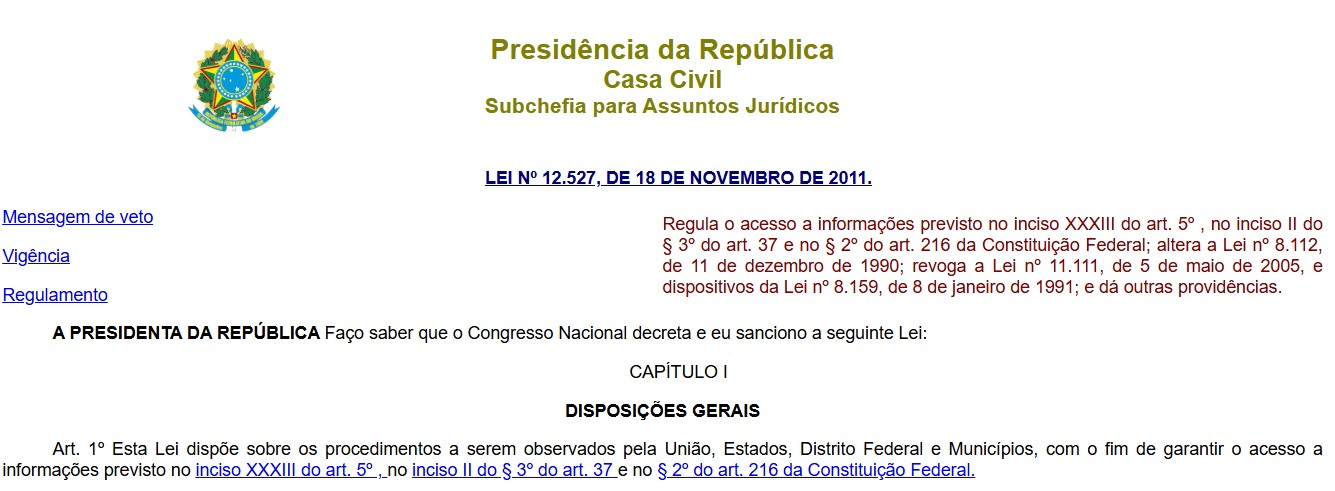
\includegraphics[width=\textwidth]{Figuras/lei-acesso-informacao}
  %\declaracaodevalidacao{validacao.pdf} % este comando deve vir por último, nos anexos
\end{document}
